% David Koch

\documentclass[
	headings=optiontotocandhead,% Erweiterung für das optionale Argument der
	% Gliederungsbefehle aktiviert.
	oneside,
	numbers=noenddot,% Keine Punkte am Ende der Gliederungsnummern und davon
	% abgeleiteten Nummern
	toc=flat, %Flache TOC --- kann man anpassen (auskommentieren)
	10pt, % Schriftgröße
	parskip=full, % Abstand zwischen Absätzen (ganze Zeile)
	listof=totoc, % Verzeichnisse im Inhaltsverzeichnis aufführen
	listof=flat, % mehr Abstand für grosse Zahlen
	numbers=noenddot, % kein Punkt am Ende bei Nummern
	%%enlargefirstpage,% Gibt es bei scrartcl nicht!!!!
	bibliography=totoc, % Literaturverzeichnis im Inhaltsverzeichnis aufführen
	%index=totoc, % Index im Inhaltsverzeichnis aufführen
	%captions=tableheading, % Beschriftung von Tabellen für Ausgabe oberhalb
	% der Tabelle formatieren
	%draft % Status des Dokuments (final/draft) draft hinzufügen zum anziegen
	%%der zeilen ende
	a4paper,DIV=14,
	% captions=tablesignature,
]{scrartcl}

\setcounter{secnumdepth}{3}

\usepackage[T1]{fontenc}
\usepackage[utf8]{inputenc}

\usepackage[english, ngerman]{babel, varioref} % your native language must be the last one!!

\usepackage{lastpage}
\usepackage{listings}
\usepackage{blindtext}

%% Aufzählungen nicht so weit einrücken
\usepackage[inline]{enumitem}
%\setitemize{leftmargin=*}
% Listen etwas wenige einrücken, erfordert enumitem
\setitemize{labelindent=2em,labelsep=0.5cm,leftmargin=12ex}

\usepackage{lmodern}

\usepackage{xspace}

\usepackage{graphicx}
\graphicspath{ {../assets} {../assets/Management} }

%%? \usepackage{textcomp}
\usepackage[hyphens]{url}
\usepackage{makeidx}
\makeindex
%%? \usepackage{graphicx}
\usepackage[numbers]{natbib}
\PassOptionsToPackage{normalem}{ulem}
\usepackage{ulem}

\usepackage{needspace}

\setlength\partopsep{0.5ex}%schoenere Listen
\usepackage[bottom]{footmisc}%fussnote ganz unten

\usepackage[]{microtype}
\UseMicrotypeSet[protrusion]{basicmath} % disable protrusion for tt fonts

\usepackage{multirow}   % Allows table elements to span several rows.
\usepackage{booktabs}   % Improves the typesettings of tables.
\usepackage{subcaption} % Allows the use of subfigures and enables their referencing.
\usepackage[ruled,linesnumbered]{algorithm2e} % Enables the writing of pseudo code.
\usepackage[usenames,dvipsnames,table]{xcolor} % Allows the definition and use of colors. This package has to be included before tikz.
\usepackage{nag}       % Issues warnings when best practices in writing LaTeX documents are violated.
\usepackage{todonotes} % Provides tooltip-like todo notes.
\usepackage{placeins}

\usepackage{color}
\usepackage[binary-units]{siunitx}

%% Override default figure placement To be within the flow of the text rather
%% than on it's own page.
% \usepackage{float}
% \makeatletter
% \def\fps@figure{H}
% \makeatother

%% bei vielen Bildern o.ä sinnvoll: Seite muss nicht bis ganz unten gefüllt werden
% \raggedbottom

%\usepackage{footbib} %  footcite, needs other tooling
%% for pandoc2 images
\makeatletter
\def\maxwidth{\ifdim\Gin@nat@width>\linewidth\linewidth\else\Gin@nat@width\fi}
\def\maxheight{\ifdim\Gin@nat@height>\textheight\textheight\else\Gin@nat@height\fi}
\makeatother
% Scale images if necessary, so that they will not overflow the page
% margins by default, and it is still possible to overwrite the defaults
% using explicit options in \includegraphics[width, height, ...]{}
\setkeys{Gin}{width=\maxwidth,height=\maxheight,keepaspectratio}

%% bessere Suche im PDF
\input{glyphtounicode}
\pdfgentounicode=1
%%%%%%%%%%%%%%%%%%%%%%%%%%%%%%%%%%%%%%%%%%%%%%%%%%%%%%%%%%%%%%%%%%%%%%%%%%%%%%%%%%

%  Kopf und Fußzeilen -- links und rechts verschieden
\newcommand{\kopfbild}{\voffset7mm
\includegraphics[width=25mm]{HTL3RLogo}}
\newcommand{\kopfHTL}{\sffamily{\textbf{\large{Projekthandbuch HTL3R}}}}

\usepackage[automark,footsepline,plainfootsepline]{scrlayer-scrpage}
\setkomafont{pageheadfoot}{\normalcolor\footnotesize\scshape}
\setkomafont{pagenumber}{\normalfont\normalsize}
\clearpairofpagestyles
\ihead{\headmark}
\ihead{\kopfbild}
\ohead{\kopfHTL}
\ifoot{\smaller{Höhere Technische Bundeslehranstalt Wien 3 | Rennweg 89b | 1030 Wien | \textcolor{orange}{www.htl.rennweg.at}}}
\ofoot{Seite \pagemark/\pageref{LastPage}}
\ModifyLayer[addvoffset=-.6ex]{scrheadings.foot.above.line}% Linie verschieben
\ModifyLayer[addvoffset=-.6ex]{plain.scrheadings.foot.above.line}% Linie verschieben
\setlength{\headheight}{32pt}

% alle Seiten mit Kopfzeile
%\renewcommand{\chapterpagestyle}{scrheadings}

%% Code Beispiele
%% eine Variante
\usepackage{listings}
\renewcommand{\lstlistingname}{\inputencoding{utf8}Listing}

\usepackage{tabularx}
\usepackage{scrhack}

\usepackage{array}
\newcommand\Tstrut{\rule{0pt}{3.2ex}}         % = `top' strut
\newcommand\Bstrut{\rule[-1.5ex]{0pt}{0pt}}   % = `bottom' strut

\newenvironment{nstabbing}
	{\setlength{\topsep}{-\parskip}
		\setlength{\partopsep}{-\parskip}
		\tabbing}
	{\endtabbing}

\usepackage{titlesec}
% \titleformat{?Überschriftenklasse?}[Absatzformatierung?]{?Textformatierung?} {?Nummerierung?}{?Abstand zwischen Nummerierung und Überschriftentext?}{?Code vor der Überschrift?}[?Code nach der Überschrift?]
\titleformat{\section}[hang]{\Large\bfseries\sffamily}{\thesection\quad}{-1.2ex}{}
\titleformat{\subsection}[hang]{\large\bfseries\sffamily}{\thesubsection\quad}{-1.2ex}{}
\titleformat{\subsubsection}[hang]{\large\bfseries\sffamily}{\thesubsubsection\quad}{-1.2ex}{}
\titleformat{\paragraph}[hang]{\large\bfseries\sffamily}{\theparagraph\quad}{-1.2ex}{}

% \titlespacing{?Überschriftenklasse?}{?Linker Einzug?}{?Platz oberhalb?}{?Platz unterhalb?}[?rechter Einzug?]
\titlespacing{\section}{0pt}{6pt}{6pt}
\titlespacing{\subsection}{0pt}{6pt}{0pt}
\titlespacing{\subsubsection}{0pt}{6pt}{0pt}
\titlespacing{\paragraph}{0pt}{6pt}{0pt}

%% sollte das letzte Package sein
\usepackage[unicode=true,
bookmarks=true,bookmarksnumbered=false,bookmarksopen=false,
breaklinks=true,pdfborder={0 0 0},backref=false,colorlinks=false]
{hyperref}
\hypersetup{pdftitle={Fenrir Management Review vom 24.09.24},
	pdfauthor={Koch, Uhlig, Burger, Vogler},
	pdfsubject={Diplomarbeit},
	pdfkeywords={5CN, DA, Fenrir}}
\urlstyle{same} % don't use monospace font for urls

% Auch Fußnoten bündig ausrichten
\deffootnote[]{1em}{1em}{\textsuperscript{\thefootnotemark\ }}
%% setup
\sloppy % weniger Meldungen
\voffset7mm % etwas nach unten

%%%%%%%%%%%%%%%%%%%%%%%%%%%%%%%%%%%%%%%%%%%%%%%%%%%%%%%%%%%%%%%%%%%%%%%%%%%%%%%%%%
\begin{document}
%% schöner: 10000 -- gar keine, 1000 als Mittelweg
\clubpenalty = 10000 % Schusterjungen verhindern
\widowpenalty = 10000 % Hurenkinder verhindern
\displaywidowpenalty = 1000

{\sffamily{\textbf{\LARGE{\textcolor{orange}{Management Review}}}}}\\
\noindent\rule{\textwidth}{0.1pt}
\begin{nstabbing}
	\hspace{4cm}\=\hspace{4cm}\=\hspace{4cm}\=\kill
	Projekttitel: \> \textbf{Fenrir}\\
	Auftraggeber: \> \textbf{Christian Schöndorfer}\\
	Auftragnehmer: \> \textbf{David Koch}\\
	Schuljahr: \> \textbf{2024/25}
	\> Klasse: \> \textbf{5CN}\\
\end{nstabbing}
{\smaller
	\begin{tabularx}{\textwidth}{l l l l}
	\hline
	\textbf{Version} & \textbf{Datum} & \textbf{Autorin/Autor} & \textbf{Änderung}\Tstrut  \\
	v1.0 & 24.09.2024 & David Koch & Erstellung des Management Reviews\Bstrut  \\
	\hline
	\end{tabularx}
}

\section{Projektstatus}
\textbf{Berichtszeitraum: 11.09.2024 bis 24.09.2024}

AAAAAAAA
Über die Sommerferien wurde bereits ein großes Stück Gesamtarbeit der Diplomarbeit verrichtet. Die Website wurde von Grund auf von uns designed, anschließend umgesetzt und läuft nun bereits unter der von easyname gesponsorten Domain \url{fenrir-ot.at}. Die Provisionierung der virtualisierten IT-Geräte der Topologie auf der UCS wurde mittels Terraform und Packer in vSphere ermöglicht. Der OT-Prototyp steht, funktioniert einwandfrei und repräsentiert eine vereinfachte Version der zweiten Betriebszelle. Mehr Informationen zu der bereits erledigten Arbeit sowie der aufgetretenen Probleme finden Sie weiter unten.

Derzeitiger Ampelstatus: Grün

\textbf{Termine}

{\smaller
	\begin{tabularx}{\textwidth}{|X|X|X|X|X|}
		\hline
		\textbf{\% abgeschlossen} & \textbf{Projektstatus} & \textbf{Erwartetes\newline Projektende} & \textbf{Geplantes Projektende} & \textbf{Abweichung} \\
		\hline
		- & - & - & - & - \\
		\hline
	\end{tabularx}
}
% \% abgeschlossen = Prozentwert, wie viel des Gesamtprojektes abgeschlossen ist. Ermittlung auf der Basis der abgeschlossenen Arbeiten (Stunden) im Verhältnis zu den noch zu erledigenden Arbeiten (in Stunden)

\textbf{Kosten}

{\smaller
	\begin{tabularx}{\textwidth}{|X|X|X|X|X|}
		\hline
		\textbf{Ist-Kosten} & \textbf{Restkosten} & \textbf{Erwartete\newline Gesamtkosten} & \textbf{Plankosten} & \textbf{Abweichung} \\
		\hline
		- & - & - & - & - \\
		\hline
	\end{tabularx}
}
% Ist-Kosten = bisher angefallene Kosten in € / bisher angefallene Stunden \\
% Restkosten = welche Kosten bzw. wieviel Stunden sind ab heute bis zum Projektende noch zu erwarten \\
% Erwartete Gesamtkosten = Ist-Kosten + Restkosten bzw. Ist-Aufwand (h) + Restaufwand (h) \\
% Plankosten = ursprünglich (Projektbeginn, Angebot) berechnete Kosten bzw. ursprünglich geschätzter Stundenaufwand \\
% Abweichung = Erwartete Gesamtkosten – Plankosten in € bzw. Erwarteter Gesamtaufwand – Planaufwand (h) \\

\textbf{Stunden}

{\smaller
	\begin{tabularx}{\textwidth}{|X|X|X|X|X|}
		\hline
		\textbf{Ist-Aufwand} & \textbf{Restaufwand} & \textbf{Erwarteter\newline Gesamtaufwand} & \textbf{Planaufwand} & \textbf{Abweichung} \\
		\hline
		- & - & - & - & - \\
		\hline
	\end{tabularx}
}
% Analog zu den Kosten (siehe oben)

\subsection{Teammotivation \colorbox{green!30}{:)}} 
Die Motivation ist im gesamte Team hoch, es bestehen jedoch Sorgen, dass durch zunehmenden Stress im Schuljahr die Arbeitszeit für die Diplomarbeit beeinträchtigt werden kann.

\section{Probleme im Projekt}
Beim Aufbau der Prototyp-Betriebszelle sind der Wasserfüllstandsensor sowie der RaspberryPi beschädigt worden (bei beiden ein Totalschaden). Die Ersatzbauteile wurden bereits bestellt und verbaut, somit besteht keine Beeinträchtigung des Projektablaufs, es bleiben mit diesen Schäden jedoch mehr Kosten offen.

Ebenfalls gab es einige Startschwierigkeiten mit vSphere und Terraform/Packer. Es wurde sich mit Viktor Kreuzer und Bernd Reither in Verbindung gesetzt um noch fehlende Berechtigungen, solche wie die Provisionierung von Distributed-Switches, zu verteilen. Die Provisionierung von Ubuntu-Server VMs lief anfangs aufgrund des fehlenden Verständnisses von Cloud-Init und co. ebenfalls nicht glatt, jedoch wurde mittlerweile eine angemessene Lösung gefunden. Windows-Server Provisionierung bleibt jedoch noch ein Knackpunkt.

Einige Bestandteile die für die OT eingeplant waren, gibt es in einer Ausführung, wie von uns gewünscht, nicht zu kaufen. Deshalb hat sich Gabriel Vogler einen 3D-Drucker zugelegt. Der Drucker kam jedoch mit einem Softwarefehler, weshalb er sich höhenmäßig nicht korrekt einstellen ließ und sich im Anschluss auch selbst beschädigt hat. Zahlreiche Versuche, den Drucker zum Laufen zu bringen, kosteten insgesamt ca. 8 Stunden. Er musste anschließend eingeschickt werden und es wurde bereits ein zuverlässigeres, moderneres Modell bestellt, was die nächsten Tage eintreffen sollte.

\subsection{Problemlösungsstrategie}
Fast alle im Projekt bisher aufgetretenen Probleme wurden bereits gelöst, somit ist keine allgemeine Problemlösung notwendig. Für noch ungelöste Probleme bezüglich der Windows-Server Provisionierung wird der in diesem Feld tätige Markus Burger, Verwandter von Julian Burger, befragt. Dieser hat ebenfalls auch schon in der Vergangenheit auf Fragen bezüglich Terraform/Packer geantwortet.

\subsection{Handlungsbedarf seitens des Managements}
Notwendiger Handlungsbedarf seitens des Managements liegt in folgenden Punkten:

\begin{enumerate}
	\item Agenda für das Diplomarbeits-Statusmeeting erstellen und rechtzeitig an alle Teilnehmer ausschicken
	\item Diplomarbeitsantrag bis zum 30.09.2024 in die elektronische DA-Datenbank hochladen
\end{enumerate}

\section{Erledigte Arbeiten (vollständig)}
\begin{table}[h]
	\begin{tabularx} {\textwidth} {
			|>{\hsize=.12\hsize}X
			|>{\hsize=.08\hsize}X
			|>{\hsize=.34\hsize}X
			|>{\hsize=.10\hsize}X
			|>{\hsize=.12\hsize}X
			|>{\hsize=.12\hsize}X
			|>{\hsize=.09\hsize}X|
		}
		
		\hline
		\rowcolor[HTML]{D9D9D9} 
		\textbf{\normalsize{Bearbeiter}} & \textbf{\normalsize{PSP-Code}} & {\textbf{\normalsize{Tätigkeit}}} & \textbf{\normalsize{Ort}} & \textbf{\normalsize{Dauer geplant (h)}} & \textbf{\normalsize{Dauer benötigt (h)}} & \textbf{\normalsize{Status}} \\ \hline
		Alle & 1.1.1.1 & Umfang erfassen & - & ? & ? & \cellcolor{green!30} \\ \hline
		Alle & 1.1.1.2 & Betreuer onboarden & - & ? & ? & \cellcolor{green!30} \\ \hline
		Alle & 1.1.1.3 & Mögliche Sponsoren/Partner erfassen & - & ? & ? & \cellcolor{green!30} \\ \hline
		Bastian Uhlig & 1.1.2.1 & Projektidee definieren & - & ? & ? & \cellcolor{green!30} \\ \hline
		David Koch & 1.1.2.2 & Provisorische Projektziele definieren & - & ? & ? & \cellcolor{green!30} \\ \hline
		Gabriel Vogler & 1.1.2.3 & Stakeholder analysieren & - & ? & ? & \cellcolor{green!30} \\ \hline
		David Koch & 1.1.2.4 & Risikos analysieren & - & ? & ? & \cellcolor{green!30} \\ \hline
		Bastian Uhlig & 1.1.2.5 & Spielregeln definieren & - & ? & ? & \cellcolor{green!30} \\ \hline
		Alle & 1.1.2.6 & Ansuchen schreiben & - & ? & ? & \cellcolor{green!30} \\ \hline
		Alle & 1.1.2.7 & Antrag schreiben & - & ? & ? & \cellcolor{green!30} \\ \hline
		David Koch & 1.2.1.1 & OSP erstellen & - & ? & ? & \cellcolor{green!30} \\ \hline
		David Koch & 1.2.1.2 & PSP erstellen & - & ? & ? & \cellcolor{green!30} \\ \hline
		Julian Burger & 1.3.2.3 & Provisionierung planen & - & ? & ? & \cellcolor{green!30} \\ \hline
		Julian Burger & 1.4.2.1 & Terraform und Packer können sich zum vSphere-Client verbinden & - & ? & ? & \cellcolor{green!30} \\ \hline
		Julian Burger & 1.4.2.2 & Packer kann eine Ubuntu-Server-VM als Template provisionieren & - & ? & ? & \cellcolor{green!30} \\ \hline
		Julian Burger & 1.4.2.3 & Terraform kann aus der Template von Packer eine VM aufsetzen & - & ? & ? & \cellcolor{green!30} \\ \hline
		Julian Burger & 1.4.2.4 & Es kann eine Bastion VM provisioniert werden & - & ? & ? & \cellcolor{green!30} \\ \hline
		Julian Burger & 1.4.2.5 & Über die Bastion können andere VMs leichter provisioniert werden & - & ? & ? & \cellcolor{green!30} \\ \hline
		Julian Burger & 1.5.1.1 & Webdesign festlegen & - & ? & ? & \cellcolor{green!30} \\ \hline
		David Koch & 1.5.1.2 & Randinformationen der technischen Umsetzung festlegen & - & ? & ? & \cellcolor{green!30} \\ \hline
		David Koch & 1.5.1.3 & easyname kontaktieren & - & ? & ? & \cellcolor{green!30} \\ \hline
		David Koch & 1.5.1.4 & Webinhalte schreiben & - & ? & ? & \cellcolor{green!30} \\ \hline
		Julian Burger & 1.5.1.5 & Website zusammenfügen & - & ? & ? & \cellcolor{green!30} \\ \hline
		David Koch & 1.5.2.1 & Instagram-Konto erstellen & - & ? & ? & \cellcolor{green!30} \\ \hline
		David Koch & 1.5.2.2 & Inhalte für Instagram desginen & - & ? & ? & \cellcolor{green!30} \\ \hline
		David Koch & 1.5.2.3 & Für das Instagram-Konto werben & - & ? & ? & \cellcolor{green!30} \\ \hline
		Bastian Uhlig & 1.5.3.1 & Fenrir-Sticker designen & - & ? & ? & \cellcolor{green!30} \\ \hline
		Bastian Uhlig & 1.5.3.2 & Sticker bestellen & - & ? & ? & \cellcolor{green!30} \\ \hline
		Bastian Uhlig & 1.5.3.3 & Sticker an Interessierte ausgeben & - & ? & ? & \cellcolor{green!30} \\ \hline
	\end{tabularx}
\end{table}

Die während den Sommerferien erledigten Arbeiten bestehen hauptsächlich aus dem Aufbau der Prototyp-Betriebszelle (inklusive dem Anlernen der Grundlagen bezüglich der Programmierung und Steuerung von Bussystemen wie OneWire, I2C und Modbus), der Einrichtung von vSphere-Provisionierung mittels Terraform auf der UCS (in Kooperation mit dem Diplomarbeitsteam Atropos) und die Erstellung einer Golden-Image-Pipeline mittels HCL-Packer (Bastion-Host, Security-Modell), sowie der Erstellung der Diplomarbeits-Website. Diese ist bereits unter der URL \url{https://www.fenrir-ot.at/} erreichbar. Die Website wurde mit dem Svelte-Framework und der Tailwind-CSS Bibliothek erstellt und mithilfe von Vite zu eine "'Static-Site"' generiert. Das Design wurde in Figma erstellt.

Der Prototyp hat zurzeit zwei Wassertanks, wobei einer befüllt wird und der andere nicht. Beide haben unten eine abgedichtete Öffnung, die in ein durchsichtigen Schlauch führt, welcher die zwei Tanks anschließend mit einer 12V Wasserpumpe dazwischen verbindet. Im ersten Tank befindet sich ein Füllstandsensor und sobald der Tank voll ist, schaltet die SPS die Pumpe ein. Diese bleibt eingeschaltet bis der erste Tank leer ist. Außerdem haben beide Wassertanks einen Temperatursensor, der auch mittels der SPS ausgelesen werden kann. Der gesamte Prototyp steht auf einem selbst gebautem Holzgerüst. Als SPS dieser Betriebszelle wird ein RaspberryPi mit der OpenPLC Runtime verwendet, welche wiederum mittels Leiterdiagramm-Programmierung programmiert worden ist.

Die zuvor bestellten 300 Stück an Fenrir-Sticker sind vom Printshop fertiggestellt und vom Projektteam bereits abgeholt worden. Die Austeilung der Sticker an Interessierte findet derzeit (und vorraussichtlich bis zum Projektende) statt.

\begin{figure}[h]
	\centering
	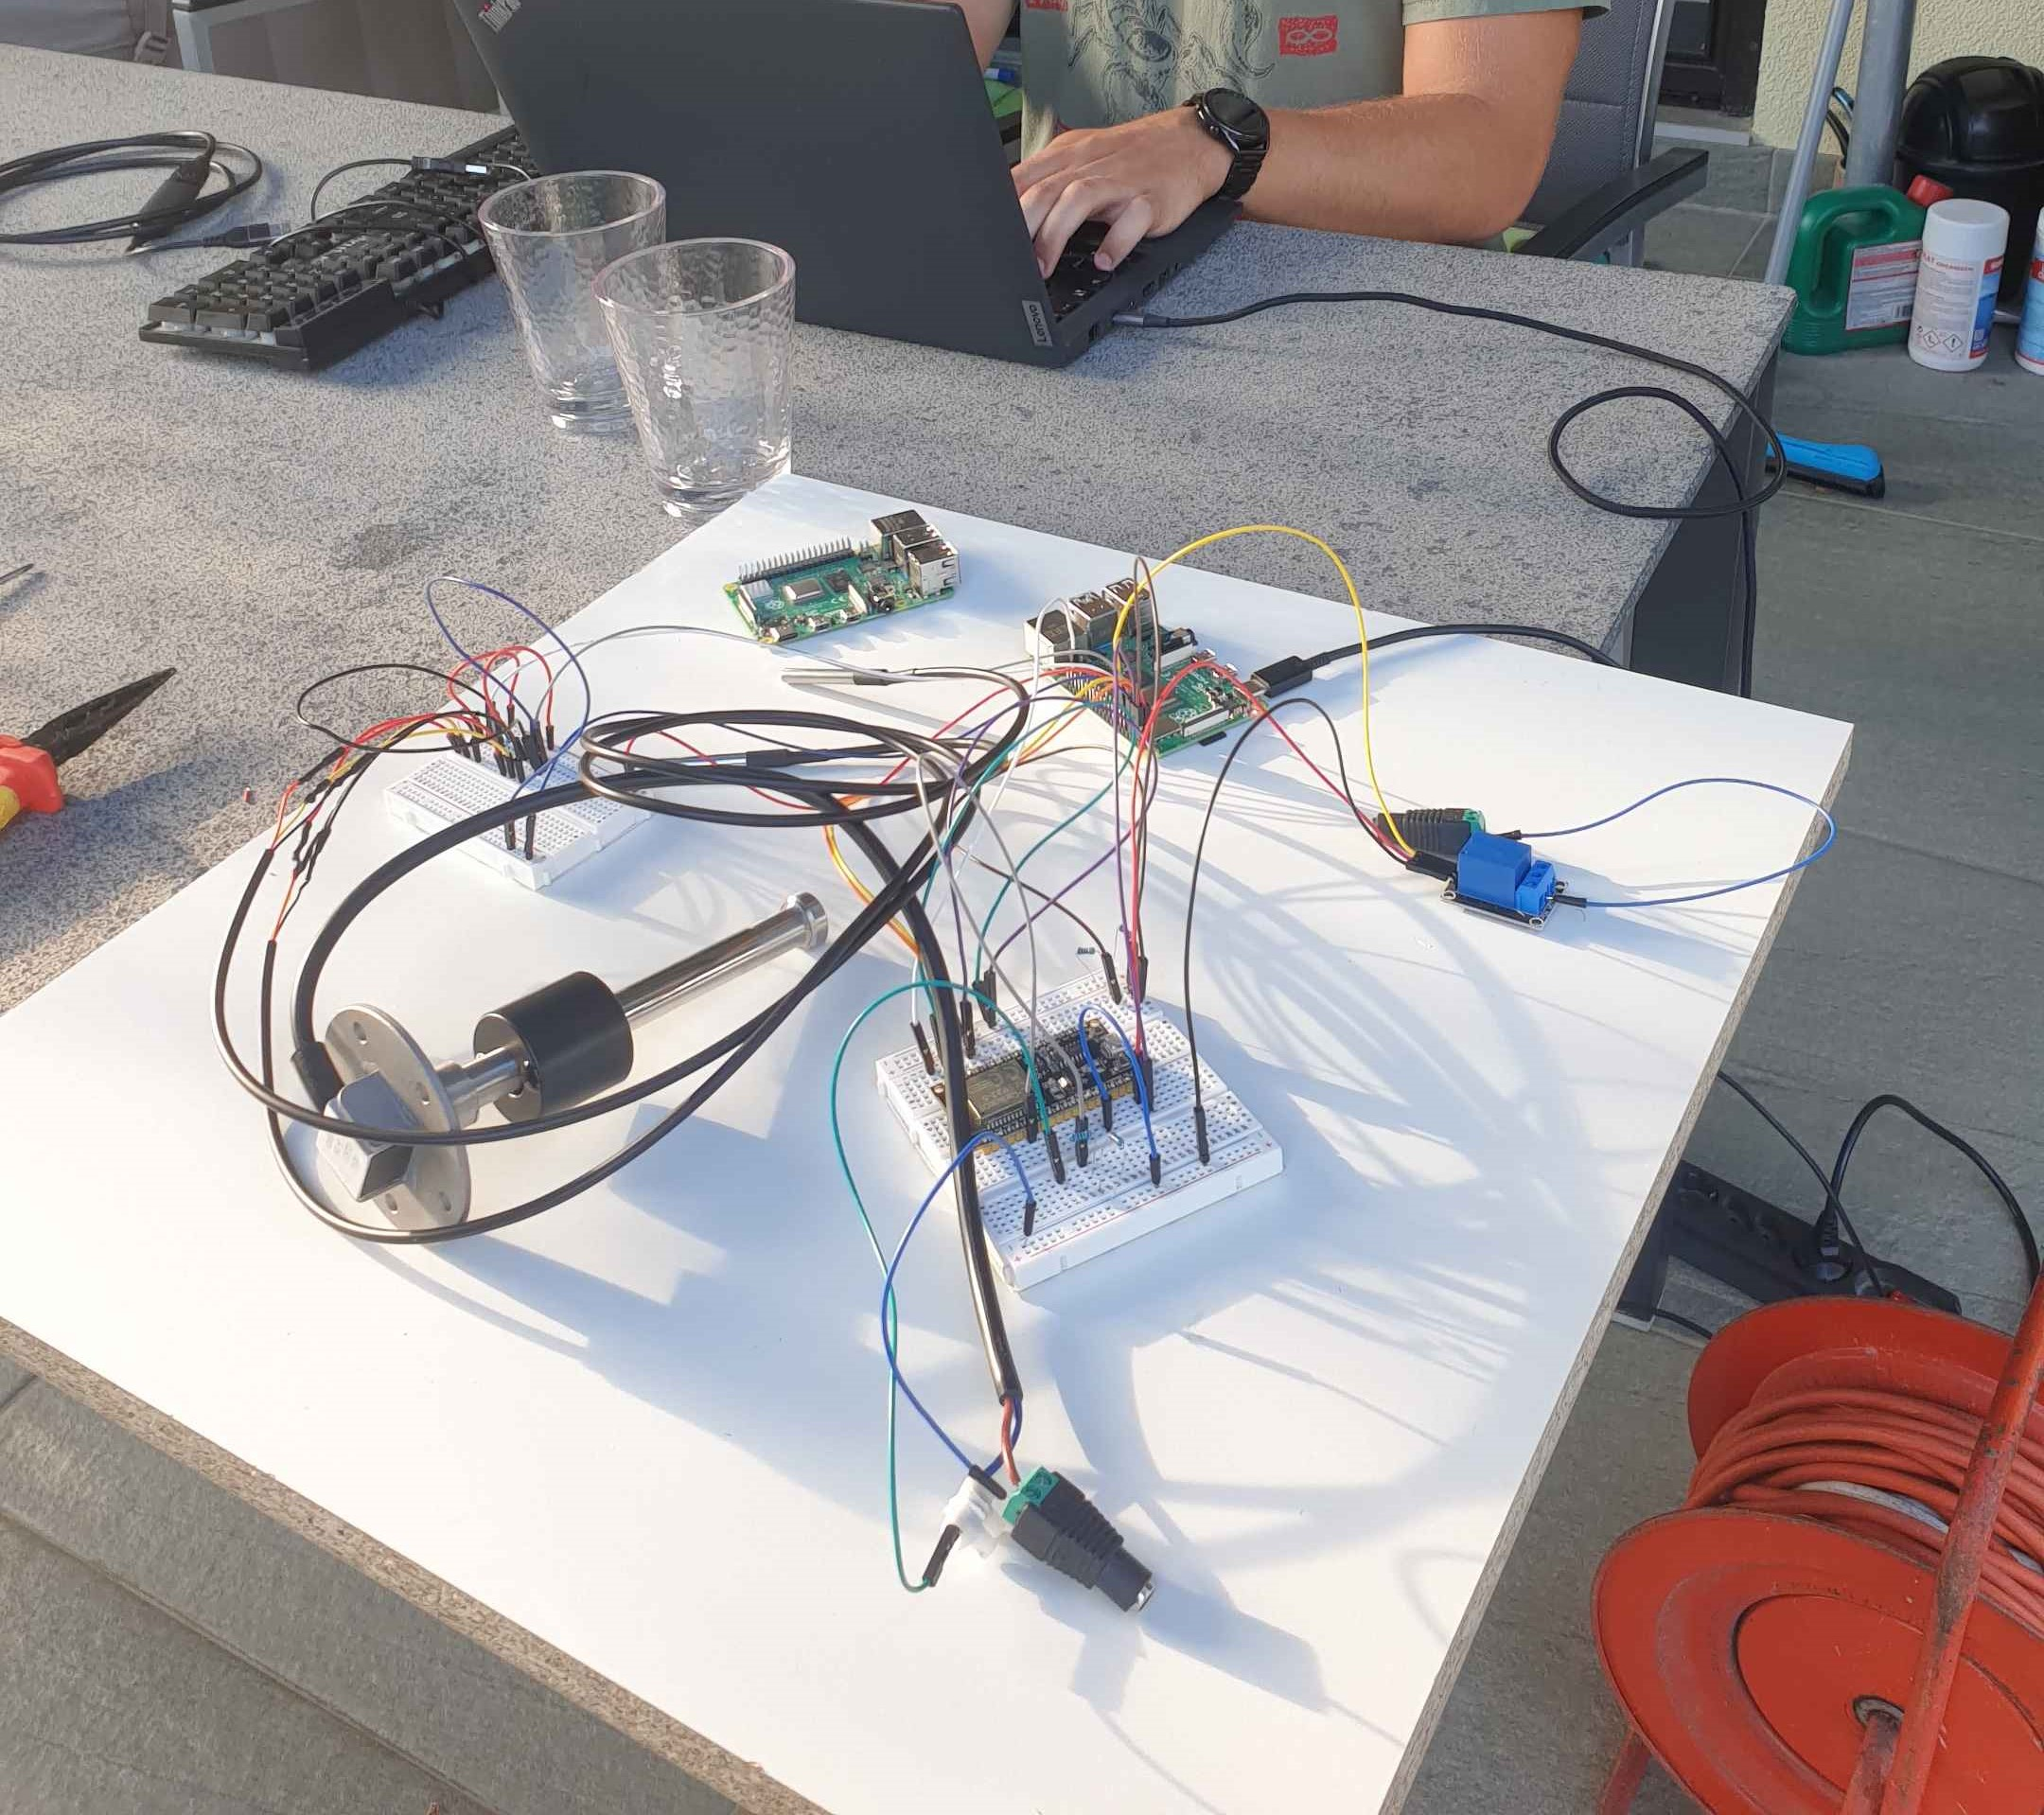
\includegraphics[width=0.6\linewidth]{20240910_1}
	\caption[]{3D-gedruckte Förderschnecke mit ihrer Hülle}
\end{figure}
\FloatBarrier 

\section{Anstehende Arbeiten}
\begin{table}[h]
	\begin{tabularx} {\textwidth} {
			|>{\hsize=.12\hsize}X
			|>{\hsize=.08\hsize}X
			|>{\hsize=.54\hsize}X
			|>{\hsize=.12\hsize}X
			|>{\hsize=.15\hsize}X|
		}
		
		\hline
		\rowcolor[HTML]{D9D9D9} 
		\textbf{\normalsize{Bearbeiter}} & \textbf{\normalsize{PSP-Code}} & {\textbf{\normalsize{Tätigkeit}}} & \textbf{\normalsize{Dauer geplant (h)}} & \textbf{\smaller{Fertigstellung geplant}} \\ \hline
		- & - & - & - & - \\ \hline
	\end{tabularx}
\end{table}

Die zuvor erstellten Planungsdokumente müssen mit den über die Sommerferien erhaltenen Informationen bezüglich des Projektumfangs überarbeitet werden. Wie zuvor erwähnt muss bis zum 20.09.2024 der Diplomarbeitsantrag offiziell abgeschickt werden, somit sollten spätestens eine Woche zuvor (am 13.09.2024) beide Diplomarbeitsbetreuer eine beinahe fertige Kopie erhalten, um diese auf Fehler zu überprüfen. Da im Antrag die Zieldefinition und im weiteren des PSP und OSP im Ganzen enthalten sind hat die Fertigstellung/Überarbeitung dieser -- im Vergleich zu den restlichen Planungsdokumenten -- die höchste Priorität.

Der Aufbau der nächsten OT-Betriebszelle beginnt, sobald der vom Kollegen Vogler bestellte 3D-Drucker ankommt und eine maßgeschneiderte Förderschnecke drucken kann.

Es muss auch eine dedizierte VPN-Verbindung zum Kollegen Vogler nach Hause erstellt werden, um jederzeit auf die bestehende OT-Gerätschaft zugreifen zu können, als auch um diese später mit virtuellen Maschinen auf der UCS verbinden zu können.

\end{document}